\subsection{信号的概念}

\begin{definition}[信号]
    \bd{信号}是人对物理世界的一种\bd{观察}。
    \bd{观察}是人通过\bd{传感器}对物理世界的一种\bd{测量}。
    \bd{传感器}是把一种物理变化转换成另一种物理变化的装置。
    \bd{测量}是指用一种物理量来表示另一种物理量。

    信号是反映(或载有)信息的物理量,是系统直接进行加工、变换以实现通信的对象。
    信号是信息的表现形式,信息则是信号里所蕴含的内容
\end{definition}

\begin{example}[传感器]
    传感器的种类繁多。例如:
    \begin{enumerate}
        \item 光
            \begin{itemize}
                \item 数码相机:光能产生电信号。
            \end{itemize}
        \item 空气振动
            \begin{itemize}
                \item 麦克风:空气的振动能产生电信号。
            \end{itemize}
        \item 温度
            \begin{itemize}
                \item 热敏电阻:阻值随温度变化。
                \item 热电偶:由对温度反应不同的两种金属制成,温差导致电压。
            \end{itemize}
    \end{enumerate}

    除此之外,还有加速度传感器、压力传感器、流量传感器等。
    值得注意的是,耳朵(图 \ref{fig:ear})就是一种传感器。
    \begin{figure}[H]
        \centering
        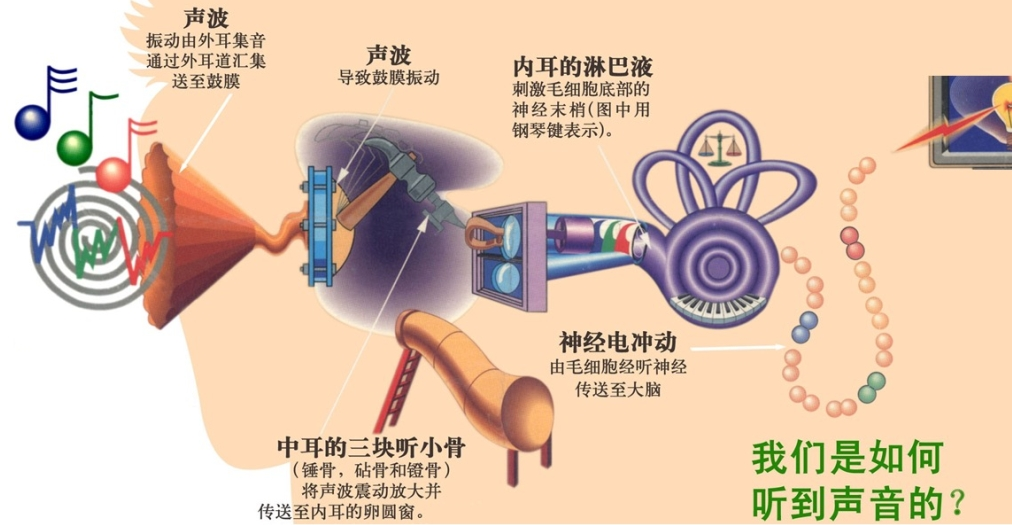
\includegraphics[width=0.5\textwidth]{chap1/img/ear.png}
        \caption{耳朵是一种传感器}
        \label{fig:ear}
    \end{figure}
\end{example}

\begin{definition}[信号处理]
    \bd{信号处理}是对信号进行变换、分析和综合等处理过程的统称。
    信号处理的目的是
    \begin{itemize}
        \item 去伪存真:去除信号中冗余的和次要的成分。
        \item 特征抽取:把信号变成易于进行分析和识别的形式。
        \item 编码解码:把信号变成易于传输、交换与存储的形式(编码),
            或从编码信号中恢复出原始信号(解码)。
    \end{itemize}
\end{definition}

\begin{example}[数字信号处理(DSP)系统]
    由于数字系统的工作具有\bd{可预测性}和\bd{可重复性},
    而模拟系统是由元器件搭建而成的电路,制造误差范围大,
    特性随温度(温度漂移)和时间变化(老化)。
    因此,\bd{数字信号处理(DSP)系统}应运而生。

    DSP 系统的特点有:
    \begin{itemize}
        \item 体积小,功耗低:数字系统通常由集成电路构成,这些电路可以在非常小的尺寸上集成大量的电子元件。这不仅减少了设备的体积,也降低了功耗,这对于移动终端的发展尤为重要。
        \item 有高度的灵活性:数字系统可以通过软件编程来实现多种功能,这使得它们非常灵活。修改程序中的一些语句就能修改系统的行为,而无需改变硬件。
        \item 模拟信号与数字信号的不同:
            \begin{itemize}
                \item 模拟音频以模拟电压的幅度表示声音强弱。
                \item 数字音频是有限数值表示的离散数字序列。
            \end{itemize}
    \end{itemize}
    例如,修改``抽样频率'',就可以改变数字音频音高/音速。
\end{example}
